\pagebreak
\subsection{Moment of Inertia} %\label{put a label here and uncomment}
\textbf{Name: Group 510}\\
\textbf{Date: 30/09 - 2015}

\subsubsection{Purpose}
The purpose of this test is to find the moment of inertia $I$, by measuring the motor velocity as a function of time.

\subsubsection{Setup}
\begin{figure}[H]
  \centering
	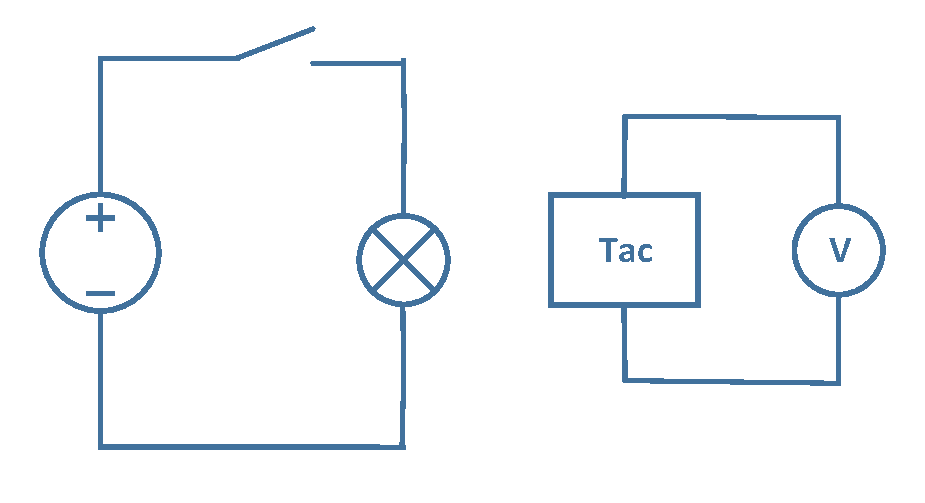
\includegraphics[scale=0.5]{figures/MotorTest7.pdf}
	\caption{Setup diagram}
\end{figure}

\subsubsection{List of Equipment}

\begin{table}[H]
\begin{tabular}{|l|l|p{4cm}|}
\hline%------------------------------------------------------------------------------------
  \textbf{Instrument}                        &  \textbf{AAU-no.}  &  \textbf{Type}       \\
\hline%------------------------------------------------------------------------------------
  Oscilloscope                               &  64672             &  Agilent DSO6034A    \\
\hline%------------------------------------------------------------------------------------
  Power Supply ($0 - 32$ V) ($0 - 10$ A)     &  77076             &  Ea - ps 7032 - 100  \\
\hline%------------------------------------------------------------------------------------
  Optical tachometer                         &  77087             &  Compact             \\
\hline%------------------------------------------------------------------------------------
\end{tabular}
\end{table}

\subsubsection{Procedure}

\begin{enumerate}
  \item Turn on the oscilloscope.
  \item On the oscilloscope press the "mode"-key choose the "normal"-option, set the trigger to "falling edge".
  \item To prevent false triggering on the oscilloscope set the trigger value to %\fxnote{input value from extracted data} mV with the turn-key.
  \item Turn on the power supply at 7 volt.
  \item Press "single"-key on oscilloscope and cut the power of the motor.
  \item Insert a USB-pin in the oscilloscope and press the save key to extract the data.
\end{enumerate}

\subsubsection{Results}

\begin{figure}[H]
	\centering
	%Trim margins @:   left        bottom       right       top
	\adjustbox{ trim = {.15\width} {.30\height} {.15\width} {.30\height}, clip }
	{
  	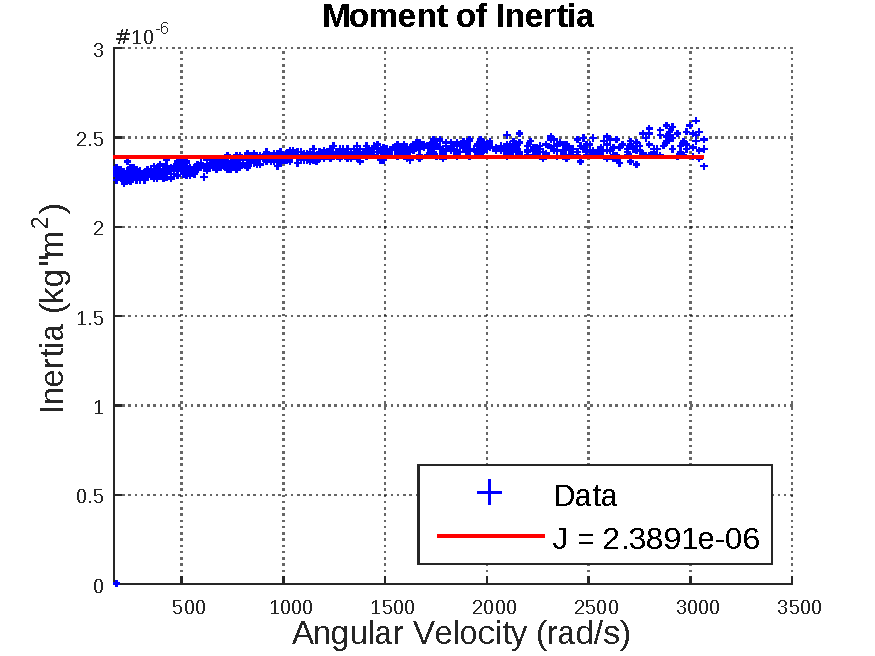
\includegraphics[width=\textwidth]{figures/momentOfInertia.pdf}
	}
	\caption{Plot of test results}
\end{figure}